
\documentclass[11pt,a4paper]{article}
\usepackage[T1]{fontenc}
\usepackage{lmodern}
\usepackage{amsmath,amssymb,amsfonts,mathtools}
\usepackage{graphicx,booktabs,longtable,array,tabularx,adjustbox}
\usepackage{geometry,microtype,fancyhdr,lastpage,etoolbox,enumitem}
\usepackage{newunicodechar,textcomp}
\usepackage{hyperref}
\hypersetup{hidelinks,pdfcreator={XeLaTeX / QM1 academic edition}}
\geometry{left=20mm,right=20mm,top=22mm,bottom=23mm}
\setcounter{secnumdepth}{2}
\setlength{\parindent}{0pt}
\setlength{\parskip}{4pt plus 1pt}
\setlength{\emergencystretch}{2em}
\setlength{\tabcolsep}{3pt}
\renewcommand{\arraystretch}{1.16}
\setlist{nosep,topsep=3pt,itemsep=2pt,leftmargin=7mm}
\AtBeginEnvironment{longtable}{\footnotesize\setlength{\tabcolsep}{2.2pt}}
\newcommand{\tightlist}{\setlength{\itemsep}{0pt}\setlength{\parskip}{0pt}}
\providecommand{\Cov}{\operatorname{Cov}}
\providecommand{\Var}{\operatorname{Var}}
\providecommand{\Corr}{\operatorname{Corr}}
\providecommand{\MAD}{\operatorname{MAD}}
\providecommand{\E}{\mathbb{E}}
\providecommand{\R}{\mathbb{R}}
\newunicodechar{—}{\textemdash}
\newunicodechar{–}{\textendash}
\newunicodechar{€}{\texteuro}
\newunicodechar{≤}{\ensuremath{\leq}}
\newunicodechar{≥}{\ensuremath{\geq}}
\newunicodechar{×}{\ensuremath{\times}}
\newunicodechar{÷}{\ensuremath{\div}}
\newunicodechar{Σ}{\ensuremath{\Sigma}}
\newunicodechar{σ}{\ensuremath{\sigma}}
\newunicodechar{μ}{\ensuremath{\mu}}
\newunicodechar{Δ}{\ensuremath{\Delta}}
\newunicodechar{∑}{\ensuremath{\sum}}
\newunicodechar{≈}{\ensuremath{\approx}}
\newunicodechar{√}{\ensuremath{\surd}}
\newunicodechar{≠}{\ensuremath{\ne}}
\newunicodechar{→}{\ensuremath{\to}}
\newunicodechar{∞}{\ensuremath{\infty}}
\newunicodechar{∈}{\ensuremath{\in}}
\newunicodechar{−}{\ensuremath{-}}
\newunicodechar{²}{\ensuremath{^{2}}}
\newunicodechar{³}{\ensuremath{^{3}}}
\newunicodechar{₀}{\ensuremath{_{0}}}
\newunicodechar{₁}{\ensuremath{_{1}}}
\newunicodechar{₂}{\ensuremath{_{2}}}
\newunicodechar{₃}{\ensuremath{_{3}}}
\newunicodechar{₄}{\ensuremath{_{4}}}
\newunicodechar{ₜ}{\ensuremath{_{t}}}
\newunicodechar{ₚ}{\ensuremath{_{p}}}
\newunicodechar{ₙ}{\ensuremath{_{n}}}
\newunicodechar{ₓ}{\ensuremath{_{x}}}
\newunicodechar{ᵢ}{\ensuremath{_{i}}}
\newunicodechar{ŷ}{\ensuremath{\hat y}}
\newunicodechar{Ŷ}{\ensuremath{\widehat Y}}
\newunicodechar{ₘ}{\ensuremath{_{m}}}
\newunicodechar{ₑ}{\ensuremath{_{e}}}
\newunicodechar{ₐ}{\ensuremath{_{a}}}
\newunicodechar{ₖ}{\ensuremath{_{k}}}
\newunicodechar{ₛ}{\ensuremath{_{s}}}
\newunicodechar{ₗ}{\ensuremath{_{l}}}
\newunicodechar{ₕ}{\ensuremath{_{h}}}
\newunicodechar{ₒ}{\ensuremath{_{o}}}
\newunicodechar{₊}{\ensuremath{_{+}}}
\newunicodechar{₋}{\ensuremath{_{-}}}
\newunicodechar{₌}{\ensuremath{_{=}}}
\newunicodechar{₍}{\ensuremath{_{(}}}
\newunicodechar{₎}{\ensuremath{_{)}}}
\newunicodechar{⁻}{\ensuremath{^{-}}}
\newunicodechar{⁺}{\ensuremath{^{+}}}
\newunicodechar{⁰}{\ensuremath{^{0}}}
\newunicodechar{¹}{\ensuremath{^{1}}}
\newunicodechar{⁴}{\ensuremath{^{4}}}
\newunicodechar{⁵}{\ensuremath{^{5}}}
\newunicodechar{⁶}{\ensuremath{^{6}}}
\newunicodechar{⁷}{\ensuremath{^{7}}}
\newunicodechar{⁸}{\ensuremath{^{8}}}
\newunicodechar{⁹}{\ensuremath{^{9}}}
\makeatletter
\renewcommand{\section}{\@startsection{section}{1}{0pt}{2.0ex plus .7ex minus .3ex}{1.0ex}{\large\bfseries}}
\renewcommand{\subsection}{\@startsection{subsection}{2}{0pt}{1.8ex plus .5ex minus .2ex}{.7ex}{\normalsize\bfseries}}
\renewcommand{\subsubsection}{\@startsection{subsubsection}{3}{0pt}{1.3ex plus .4ex minus .2ex}{.5ex}{\normalsize\bfseries}}
\makeatother
\pagestyle{fancy}
\fancyhf{}
\renewcommand{\headrulewidth}{0.35pt}
\renewcommand{\footrulewidth}{0pt}
\fancyhead[L]{\small\textsc{KEDGE Business School --- QM1}}
\fancyhead[R]{\small\textsc{2026--2027}}
\fancyfoot[L]{\small Badr ABOUFARASSE, PhD}
\fancyfoot[R]{\small\thepage\ /\ \pageref{LastPage}}
\setlength{\headheight}{14pt}
\setkeys{Gin}{keepaspectratio}
\begin{document}

\begin{center}
{\small\textsc{KEDGE Business School \quad EBP1 \quad Quantitative Methods 1}}\\[6pt]
{\Large\bfseries Worksheet 3 — Dispersion and concentration}\\[6pt]
{\normalsize\bfseries Fully worked solutions}\\[6pt]
{\small Badr ABOUFARASSE, PhD \quad --- \quad 2026--2027}
\end{center}
\vspace{2mm}\hrule\vspace{6mm}

\hypertarget{core-applications}{%
\section{Core applications}\label{core-applications}}

Master the essential definitions and calculations from the course.

\emph{Core application --- 25 min}

\hypertarget{exercise-4-medial-and-cumulative-relative-masses}{%
\subsection{Exercise 4 --- Medial and cumulative relative masses}\label{exercise-4-medial-and-cumulative-relative-masses}}

The spending of 40 customers (€) is grouped below. Approximate class monetary mass by nᵢ × class midpoint.

\begin{longtable}[]{@{}llllll@{}}
\toprule\noalign{}
Classe / Class & {[}10,20{[} & {[}20,30{[} & {[}30,40{[} & {[}40,50{[} & {[}50,60{[} \\
\midrule\noalign{}
\endhead
\bottomrule\noalign{}
\endlastfoot
nᵢ & 8 & 12 & 10 & 6 & 4 \\
\end{longtable}

\begin{enumerate}
\tightlist
\item
  Compute midpoints, masses, cumulative masses and relative cumulative mass shares.
\item
  Interpolate the medial in the class containing half of total mass.
\item
  Compute the frequency median and compare the two statistics.
\end{enumerate}

\hypertarget{fully-worked-solution}{%
\subsubsection{Fully worked solution}\label{fully-worked-solution}}

\begin{longtable}[]{@{}llllll@{}}
\toprule\noalign{}
Classe / Class & nᵢ & cᵢ & nᵢcᵢ & Masse cumulée & Masse cumulée (\%) \\
\midrule\noalign{}
\endhead
\bottomrule\noalign{}
\endlastfoot
{[}10,20{[} & 8 & 15 & 120 & 120 & 9.52 \\
{[}20,30{[} & 12 & 25 & 300 & 420 & 33.33 \\
{[}30,40{[} & 10 & 35 & 350 & 770 & 61.11 \\
{[}40,50{[} & 6 & 45 & 270 & 1040 & 82.54 \\
{[}50,60{[} & 4 & 55 & 220 & 1260 & 100 \\
TOTAL & 40 & --- & 1260 & --- & 100 \\
\end{longtable}

\[S=\sum n_ic_i=120+300+350+270+220=1260,\qquad S/2=630.\]

Half the mass lies in {[}30,40{[}, since 420 \textless{} 630 ≤ 770. With linear interpolation of the mass:

\[MI=30+\frac{630-420}{350}\times10=36\ \mathrm{euros}.\]

The frequency median is €30 (20 of 40 observations below €30). The medial, €36, divides monetary mass, not the number of observations.

\emph{Core application --- 20 min}

\hypertarget{extra-1-dispersion-from-a-frequency-table}{%
\subsection{Extra 1 --- Dispersion from a frequency table}\label{extra-1-dispersion-from-a-frequency-table}}

The number of weekly complaints per store is distributed as follows:

\begin{longtable}[]{@{}llllll@{}}
\toprule\noalign{}
Complaints x & 0 & 1 & 2 & 3 & 4 \\
\midrule\noalign{}
\endhead
\bottomrule\noalign{}
\endlastfoot
Stores n & 4 & 8 & 10 & 6 & 2 \\
\end{longtable}

\begin{enumerate}
\tightlist
\item
  Calculate the mean, population variance and standard deviation.
\item
  Calculate the coefficient of variation.
\item
  Interpret every result in context.
\end{enumerate}

\textbf{Method hint:}

Build columns nx and nx². Use E(X²) − {[}E(X){]}² for the population variance.

\hypertarget{fully-worked-solution-1}{%
\subsubsection{Fully worked solution}\label{fully-worked-solution-1}}

\textbf{Totals.} N = 30; Σnx = 0+8+20+18+8 = 54; Σnx² = 0+8+40+54+32 = 134.

\textbf{Mean.} 54/30 = \textbf{1.80 complaints}.

\textbf{Variance.} E(X²) = 134/30 = 4.4667. Therefore σ² = 4.4667 − 1.80² = \textbf{1.2267}.

\textbf{Standard deviation.} σ = √1.2267 = \textbf{1.108 complaints}.

\textbf{Coefficient of variation.} CV = 1.108/1.80 × 100 = \textbf{61.6\%}.

\textbf{Interpretation.} Stores receive 1.8 complaints on average, with substantial heterogeneity relative to that mean. The CV is meaningful here because the ratio-scale variable has a genuine zero, but comparisons should use the same observation period and definition of a complaint.

\begin{longtable}[]{@{}llll@{}}
\toprule\noalign{}
xᵢ & nᵢ & nᵢxᵢ & nᵢxᵢ² \\
\midrule\noalign{}
\endhead
\bottomrule\noalign{}
\endlastfoot
0 & 4 & 0 & 0 \\
1 & 8 & 8 & 8 \\
2 & 10 & 20 & 40 \\
3 & 6 & 18 & 54 \\
4 & 2 & 8 & 32 \\
Σ & 30 & 54 & 134 \\
\end{longtable}

\hypertarget{assessment-and-exam-practice}{%
\section{Assessment and exam practice}\label{assessment-and-exam-practice}}

Practise independently with assessment and final-exam style questions.

\emph{Assessment / exam practice --- 35 min}

\hypertarget{exercise-2-dispersion-of-grouped-data}{%
\subsection{Exercise 2 -- Dispersion of grouped data}\label{exercise-2-dispersion-of-grouped-data}}

Using the 210-customer distribution from Worksheet 2, calculate {\(\sum n_ic_i\)}, {\(\sum n_ic_i^2\)}, mean, population variance, standard deviation, coefficient of variation and IQR. Compare the information provided by standard deviation and IQR.

\hypertarget{fully-worked-solution-2}{%
\subsubsection{Fully worked solution}\label{fully-worked-solution-2}}

{\[\sum n_ic_i=6665,
\qquad
\sum n_ic_i^2=227036.5.\]} {\[\bar
x=\frac{6665}{210}\approx31.7381.\]} {\[V=\frac{227036.5}{210}-\bar
x^2\approx73.8195.\]} {\[\sigma\approx8.5918,
\qquad
CV=\frac{8.5918}{31.7381}\approx27.07\%.\]} {\[IQR=37.50-26.56\approx10.94.\]} Standard deviation uses the full distribution and is sensitive to extremes; the IQR describes the spread of the central half and is more robust.

\hypertarget{weighted-product-audit-table}{%
\subsubsection{Weighted-product audit table}\label{weighted-product-audit-table}}

\begin{longtable}[]{@{}lllll@{}}
\toprule\noalign{}
Class & n & c & n×c & n×c² \\
\midrule\noalign{}
\endhead
\bottomrule\noalign{}
\endlastfoot
{[}10,14{[} & 4 & 12 & 48 & 576.00 \\
{[}14,18{[} & 12 & 16 & 192 & 3072.00 \\
{[}18,26{[} & 32 & 22 & 704 & 15488.00 \\
{[}26,30{[} & 32 & 28 & 896 & 25088.00 \\
{[}30,35{[} & 60 & 32.5 & 1950 & 63375.00 \\
{[}35,40{[} & 35 & 37.5 & 1312.5 & 49218.75 \\
{[}40,45{[} & 25 & 42.5 & 1062.5 & 45156.25 \\
{[}45,50{[} & 5 & 47.5 & 237.5 & 11281.25 \\
{[}50,55{[} & 5 & 52.5 & 262.5 & 13781.25 \\
Σ & 210 & --- & 6665 & 227036.50 \\
\end{longtable}

\[\begin{gathered}
V=\frac{227036.5}{210}-\left(\frac{6665}{210}\right)^2=73.8195,\\\sigma=\sqrt{73.8195}=8.5918.
\end{gathered}\]

Midpoint-based variance approximates the dispersion of the unknown individual observations.

\emph{Assessment / exam practice --- 30 min}

\hypertarget{exercise-3-lorenz-curve-and-gini-coefficient}{%
\subsection{Exercise 3 -- Lorenz curve and Gini coefficient}\label{exercise-3-lorenz-curve-and-gini-coefficient}}

Income values are {\(10,12,18,25,35\)}. Calculate cumulative population and income shares, construct the Lorenz curve, calculate the area by trapezoids, derive the Gini coefficient and explain why Gini measures concentration without explaining its causes.

\hypertarget{fully-worked-solution-3}{%
\subsubsection{Fully worked solution}\label{fully-worked-solution-3}}

Total income is 100. Lorenz points are {\[(0,0),\ (0.2,0.10),\ (0.4,0.22),\ (0.6,0.40),\
(0.8,0.65),\ (1,1).\]} {\[A=0.374,
\qquad
G=1-2A=0.252=25.2\%.\]}

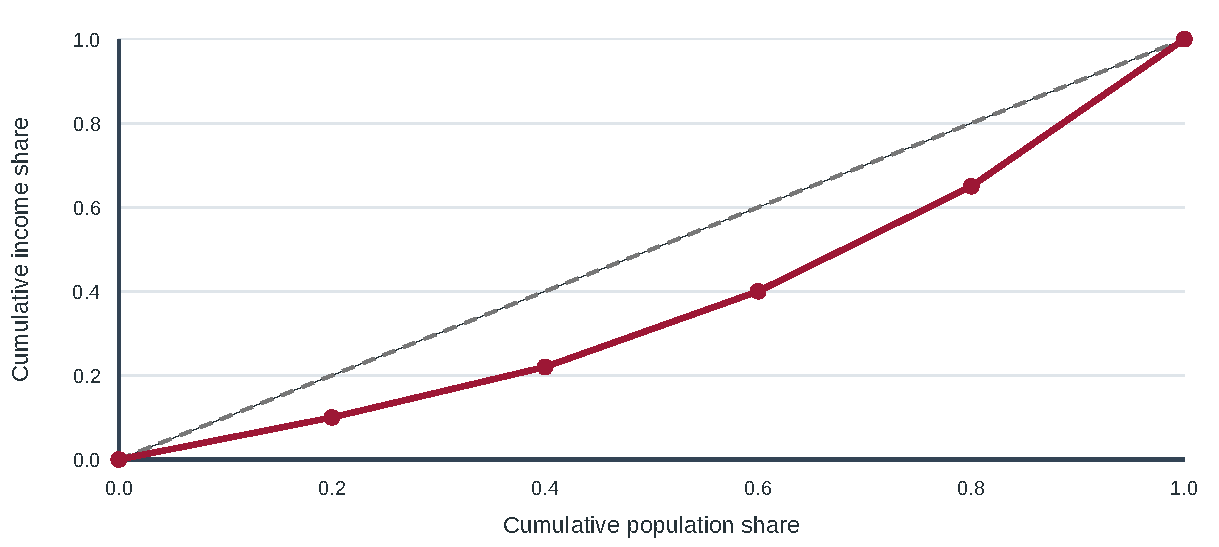
\includegraphics[width=0.85\textwidth,height=\textheight]{assets/chapter-3-solutions-en-chart-01.pdf}

\emph{Lorenz curve and equality line}

The Gini coefficient summarizes concentration; it does not identify the economic or institutional mechanisms causing it.

\hypertarget{optional-advanced-practice}{%
\section{Optional advanced practice}\label{optional-advanced-practice}}

Explore additional interpretations and professional applications.

\emph{Advanced practice --- 30 min}

\hypertarget{exercise-1-boxplot-potential-outliers-and-variance-choice}{%
\subsection{Exercise 1 -- Boxplot, potential outliers and variance choice}\label{exercise-1-boxplot-potential-outliers-and-variance-choice}}

Consider {\[5,6,6,7,7,8,8,9,9,10,11,20.\]} Use the median-of-halves convention for quartiles.

\begin{enumerate}
\item
  Calculate the five-number summary.
\item
  Calculate the range and IQR.
\item
  Calculate the fences {\(Q_1-1.5IQR\)} and {\(Q_3+1.5IQR\)} and identify potential outliers.
\item
  Calculate the mean and mean absolute deviation.
\item
  Calculate population variance and standard deviation if the 12 observations are the entire population.
\item
  Calculate sample variance and standard deviation if they are a sample.
\end{enumerate}

\hypertarget{fully-worked-solution-4}{%
\subsubsection{Fully worked solution}\label{fully-worked-solution-4}}

{\[\min=5,\qquad Me=8,\qquad
\max=20.\]} Lower half {\(5,6,6,7,7,8\)} gives {\[Q_1=\frac{6+7}{2}=6.5.\]} Upper half {\(8,9,9,10,11,20\)} gives {\[Q_3=\frac{9+10}{2}=9.5.\]} Thus {\[IQR=9.5-6.5=3.\]} The fences are {\[B_L=6.5-1.5(3)=2,
\qquad
B_U=9.5+1.5(3)=14.\]} Since {\(20>14\)}, 20 is a potential outlier. {\[\bar
x=\frac{106}{12}\approx8.8333.\]} {\[MAD=\frac1{12}\sum|x_i-\bar
x|\approx2.4722.\]} Population variance and standard deviation: {\[\sigma^2\approx14.1389,
\qquad
\sigma\approx3.7602.\]} Sample variance and standard deviation: {\[s^2\approx15.4242,
\qquad
s\approx3.9274.\]}

\hypertarget{table-of-every-deviation}{%
\subsubsection{Table of every deviation}\label{table-of-every-deviation}}

\begin{longtable}[]{@{}llll@{}}
\toprule\noalign{}
i & x & \textbar x−106/12\textbar{} & (x−106/12)² \\
\midrule\noalign{}
\endhead
\bottomrule\noalign{}
\endlastfoot
1 & 5 & 3.8333 & 14.6944 \\
2 & 6 & 2.8333 & 8.0278 \\
3 & 6 & 2.8333 & 8.0278 \\
4 & 7 & 1.8333 & 3.3611 \\
5 & 7 & 1.8333 & 3.3611 \\
6 & 8 & 0.8333 & 0.6944 \\
7 & 8 & 0.8333 & 0.6944 \\
8 & 9 & 0.1667 & 0.0278 \\
9 & 9 & 0.1667 & 0.0278 \\
10 & 10 & 1.1667 & 1.3611 \\
11 & 11 & 2.1667 & 4.6944 \\
12 & 20 & 11.1667 & 124.6944 \\
Σ & 106 & 29.6667 & 169.6667 \\
\end{longtable}

\[\sum x_i^2=1106,\quad\sum(x_i-\bar x)^2=1106-\frac{106^2}{12}=169.6667.\]

\[e=29.6667/12=2.4722,\quad \sigma^2=169.6667/12=14.1389,\quad s^2=169.6667/11=15.4242.\]

Table entries are rounded for display; use exact fractions until the final rounding.

\emph{Advanced practice --- 25 min}

\hypertarget{extra-2-comparing-concentration-and-robustness}{%
\subsection{Extra 2 --- Comparing concentration and robustness}\label{extra-2-comparing-concentration-and-robustness}}

Two markets have the following ordered firm market shares:

\begin{longtable}[]{@{}llllll@{}}
\toprule\noalign{}
Market A & 10\% & 15\% & 20\% & 25\% & 30\% \\
Market B & 2\% & 8\% & 10\% & 20\% & 60\% \\
\midrule\noalign{}
\endhead
\bottomrule\noalign{}
\endlastfoot
\end{longtable}

\begin{enumerate}
\tightlist
\item
  Construct cumulative shares for each market.
\item
  Explain which Lorenz curve is farther from equality.
\item
  For each market calculate the range and discuss why it is insufficient.
\item
  State a defensible concentration conclusion.
\end{enumerate}

\textbf{Method hint:}

With five equal-weight firms, cumulative population shares increase by 20 percentage points.

\hypertarget{fully-worked-solution-5}{%
\subsubsection{Fully worked solution}\label{fully-worked-solution-5}}

\textbf{Cumulative shares.} Market A: 0\%, 10\%, 25\%, 45\%, 70\%, 100\%. Market B: 0\%, 2\%, 10\%, 20\%, 40\%, 100\%. Population coordinates are 0\%, 20\%, 40\%, 60\%, 80\%, 100\%.

\textbf{Lorenz comparison.} At every interior population share, B's cumulative market share is lower. Its Lorenz curve is therefore farther below the equality line: B Lorenz-dominates in the direction of greater concentration.

\textbf{Ranges.} A: 30−10 = 20 points. B: 60−2 = 58 points. The range confirms a difference but uses only two firms and ignores the middle of the distribution.

\textbf{Conclusion.} Market B is clearly more concentrated: the largest firm alone controls 60\%, and the bottom 80\% of firms jointly control only 40\%. A complete report should show the Lorenz curve or a concentration index and should not infer market power from shares alone.

\end{document}
